% Created 2020-10-25 So 23:03
% Intended LaTeX compiler: pdflatex
\UseRawInputEncoding

\documentclass[11pt]{scrartcl}
\usepackage[utf8]{inputenc}
\usepackage[T1]{fontenc}
\usepackage[ngerman]{babel}
\usepackage{graphicx}
\usepackage{grffile}
\usepackage{longtable}
\usepackage{wrapfig}
\usepackage{rotating}
\usepackage[normalem]{ulem}
\usepackage{amsmath}
\usepackage{trfsigns}
\usepackage{textcomp}
\usepackage{amssymb}
\usepackage{capt-of}
\usepackage{MnSymbol}
\usepackage{mathtools}
\usepackage{setspace}
\usepackage{nicematrix}
\usepackage{pdfpages}
% \usepackage{getlab}
\usepackage{listings}
\usepackage{pdfpages}
\usepackage[straightvoltages, european resistors, european inductors]{circuitikz}
\usetikzlibrary{arrows.meta}
\tikzset{FARROW/.style={arrows={-Triangle[angle=45:2.0mm]}}}
%\usepackage{hyperref}
% \usepackage{varwidth}


\definecolor{darkspringgreen}{rgb}{0.09, 0.45, 0.27}    % Farbe für die Kommentare bei Listings
\lstset{
  language= Matlab,                     % Setzt die Sprache
  basicstyle=\scriptsize\ttfamily,     % Setzt den Standardstil
  % keywordstyle=\color{red}\bfseries,    % Setzt den Stil für Schlüsselwörter
  identifierstyle=\color{blue},        % Identifier bekommen keine gesonderte formatierung
  commentstyle=\color{darkspringgreen},        % Stil für Kommentare
  stringstyle=\ttfamily,             % Stil für Strings (gekennzeichnet mit "String")
  breaklines=true,             % Zeilen werden umgebrochen
  numbers=left,                 % Zeilennummern links
  numberstyle=\tiny,             % Stil für die Seitennummern
  frame=single,                 % Rahmen
  % backgroundcolor=\color{myGrey},     % Hintergrundfarbe
  % caption={Java-Code},             % Caption
  tabsize=2                % Größe der Tabulatoren
}



\newcommand{\GETHeader}[6]{%
  \begin{titlepage}
    \pagestyle{empty} \enlargethispage*{25cm}\samepage{
      \vspace*{-2.5cm}
      \begin{center}
        %
        \begin{tabular}[b]{lr}
          %
          \hspace*{-1.5cm}
          \begin{tabular}{p{3.8cm}}
            
\includegraphics[width=3.8cm]{./Figures/TUGraz}
          \end{tabular}
          %
          \hspace*{-1cm}
          %
          %
          \begin{tabular}{p{13.8cm}}
            \begin{flushright}
              \large
              Institut für Grundlagen und Theorie der Elektrotechnik\\
              ~\\
            \end{flushright}
          \end{tabular}
        \end{tabular}

        \vspace*{2.2cm}
        %
        \Huge {Elektrische Netzwerke und Mehrtore \\ Übung\\} %
        \vspace*{.5cm} \Large{ Wintersemester 2020\\}
        %
        \vspace*{1.5cm}

        \Huge{\textbf{#1}\\}

        %
        % \vspace*{0.8cm} \Large{Übungsdatum: {#2}\\}
        %
        \vspace*{1cm} \vfill
        %
        \Large{Gruppe: {#2}\\} \vspace*{0.5cm}%


        % \Large{Protokollführer(in): {#3}\\} \vspace*{1cm}

        \Large{Gruppenteilnehmer:\\} \vspace*{.1cm}
        % Name der beteiligten Studierenden
        \Large{#3} \vspace{1cm}
        %
        %
        \Large{Vortragende: #4\\} \vspace*{.1cm}   %\vspace*{1.5cm}
        % \Large{Betreuer(in): #6\\}
        \vspace*{1.5cm}
        %
        \Large{#5, am #6}
      \end{center}}%
    %
    \clearpage
  \end{titlepage}}








\begin{document}

\GETHeader                                                                              %  Bitte Ausfüllen!!!
% ----------------------------
{Protokoll Übung 3: \\ Schaltvorgang Kondensator}                         %  Übungstitel
% ----------------------------
% {25. Mai 2020}                                                                  %  Übungsdatum
% ----------------------------
{04}                                                                   %  Gruppen-Nr.
% ----------------------------
% {Matthias Fottner}                                                                      % Name des Protokollführers oder der Protokollführerin
% ----------------------------
{
  \begin{center}
    \begin{minipage}{0.28\linewidth}
      1. Matthias Fottner\\
      2. David Keller\\
      3. Moritz Woltron
    \end{minipage}
  \end{center}
}
% ----------------------------
{Helena Grabner}                                                                     %  Laborleiter(in)
% {Übung 2}                                                               %  Betreuer(in)
% ----------------------------
{Graz}                                                                                  %  Ort der Protokollerstellung
{\today}                                                                %  Datum Protokollerstellung


\newcommand{\unit}[1]{\,\text{#1}}


\tableofcontents

\newpage


\allowdisplaybreaks

\setlength{\jot}{10pt}

\section{Ermitteln der DGL von $i_L(t)$ für $0 \leq t \leq 2\tau_1$} %David
\subsection{Schaltbild des Netzwerks für $0 \leq t \leq 2\tau_1$}%David

\begin{figure}[!htb]
	\begin{center}
		\begin{circuitikz} [european resistors, scale=1]

			%			\clip (-2,-5.7) rectangle (12.5, 5);
			\draw(0,0) to [L=$L$, v<={\color{blue}{$u_{L}$}}, i<={\color{red}{$i_L$}}] (0,4)
			to [R=$R_1$, v<={\color{blue}{$u_{R1}$}}] ++ (4,0)
			to [vsource, v>={\color{blue}{$U_{0}$}}] ++ (0,-4)
			to [short] ++ (-4,0);
			\draw[darkspringgreen, thin, <-] (2,2)node{$m_1$}  ++(-60:0.5) arc (-60:170:0.5);


		\end{circuitikz}
	\end{center}
	\caption{Netzwerk im Zeitintervall $0 \leq t \leq 2\tau_1$.}
	\label{fig:schaltplan_a}
\end{figure}

\subsection{Aufstellen der DGL mithilfe der allgemeinen Lösungsformel} %David

Da es sich um ein LR-Netzwerk handelt, lässt sich $\tau_1$ folgendermaßen bestimmen:

\begin{equation*}
\frac{1}{\lambda} = \tau_{1} = \frac{L}{R} = \frac{100 \unit{mH}}{50 \unit{$\Omega$}} = 2 \unit{ms}
\end{equation*}

Weiters lässt sich durch einsetzen in die allgemeine Lösungsformel für Transiente Vorgänge
mit einem Energiespeicher der Strom $i_L$ für $0 \leq t \leq 2\tau_1$ ermitteln.\\

Allgemeine Lösungsformel:

\begin{equation*}
	x(t) = x_f + [ \, x_0 - x_f ] \, \cdot e^{(-\frac{t-t_0}{\tau})}
\end{equation*}

Das Bauteilgesetz der Spule besagt, dass der Strom eine stetige Größe ist, während die Spannung \glqq Sprünge\grqq{} aufweisen kann. Aufgrund dieser Tatsache, darf man die für obige Lösungsformel benötigten Werte wie folgt annehmen:

\begin{equation*}
	x_f = 0 \unit{V}
\end{equation*}

\begin{equation*}
	x_0 = U_0 = 10 \unit{V}
\end{equation*}

\begin{equation*}
	u_{R1}(0) = R_1 * I_{L_0} = 2.5 \unit{V}
\end{equation*}

Durch anschließendes Einsetzen erhält man:

\begin{equation*}
	u_L = 0 + [ \, U_0 - u_{R1}(0) - 0 ] \, \cdot e^{(-\frac{t}{\tau_1})} = [ \, 10 \unit{V} - 2.5 \unit{V} ] \, \cdot e^{(-\frac{t}{2 \unit{ms}})}
\end{equation*}

Masche $m_1$:
\begin{align*}
	u_{R_1} &= U_0 - u_L\\
	R_1 * i_L &= U_0 - u_L\\
	i_L &= \frac{U_0 - u_L}{R_1} = \frac{U_0 - (U_0 - R_1 \cdot I_{L_0}) \cdot e^{(-\frac{t}{\tau_1})}}{R_1} \\
	i_L (t = 2 \tau_1) &= \frac{10\unit{V} - (7,5 \cdot e^{(-\frac{t}{2 \unit{ms}})})}{50 \unit{$\Omega$}} = 0,2 \unit{A} - 0,15 \unit{A} \cdot e^{-(\frac{t}{2 \unit{ms}})} \\
	i_L (t = 2 \tau_1) &= 179,7 \unit{mA}
\end{align*}


\section{Ermitteln der DGL von $i_L(t)$ für $t > 2\tau_1$}%Matthias
\subsection{Schaltbild des Netzwerks für $t > 2\tau_1$}%Matthias
\begin{figure}[!htb]
\begin{center}
\begin{circuitikz}
  \draw (0,8) to[L=$L$, v={\color{blue}{$u_L$}}, i={\color{red}{$i_L$}}] (0,0)
  		to[short, -*] ++ (4,0) node[label={[font=\footnotesize]-90:n2}] {}
  		to[R=$R_2$, v={\color{blue}{$u_{R2}$}}, i={\color{red}{$i_{R2}$}}, *-*] ++ (0,8)
  		to[short] ++ (4,0)
  		to[R=$R_3$, v<={\color{blue}{$u_{R3}$}}] ++ (0,-4)
  		to[C=$C$, v<={\color{blue}{$u_C$}}, i<={\color{red}{$i_C$}}] ++ (0,-4)
  		to[short] ++ (-4,0);
  \draw (0,8) to[short] (4,8) node[label={[font=\footnotesize]90:n1}] {};
  \draw[darkspringgreen, thin, <-] (2,4)node{$m_1$}  ++(-60:0.5) arc (-60:170:0.5);
  \draw[darkspringgreen, thin, <-] (6,4)node{$m_2$}  ++(-60:0.5) arc (-60:170:0.5);
\end{circuitikz}
\end{center}
\end{figure}

\subsection{Aufstellen der Kirchhoff'schen Knoten- und Maschengleichungen}%Matthias
\begin{align*}
	n_1&: \qquad i_L - i_{R2} - i_C = 0 \\
	n_2&: \qquad i_C + i_{R2} - i_L = 0 \\ \\
	m_1&: \qquad -u_{R2} - u_L = 0 \\
	m_2&: \qquad u_{R2} - u_{R3} - u_C = 0
\end{align*}

\subsection{Herleitung der DGL 2. Ordnung von $i_L(t)$ für $t > 2\tau_1$}%Matthias
\begin{align*}
	-i_C - i_{R2} + i_L &= 0 \\
	-C {\color{darkspringgreen}{u_C}}' - \frac{u_{R2}}{R_2} + i_L &= 0 
\end{align*}
{\color{darkspringgreen}{
\begin{align*}
		u_C &= u_{R2} - u_{R3} \\
			&= -u_L - u_{R3} \\
			&= -(L i_L' + u_{R3})	
\end{align*}}}
\begin{align*}
	\Longrightarrow C \frac{d}{dt} \left[ L i_L' + u_{R3}\right] - \frac{u_{R2}}{R2} + i_L &= 0 \\
	C L i_L'' + \frac{d}{dt} C R_3 i_C - \frac{u_{R2}}{R2} + i_L &= 0 \\
	C L i_L'' + \frac{d}{dt} C R_3 (i_L - i_{R2}) - \frac{u_{R2}}{R2} + i_L &= 0 \\
	C L i_L'' +  C R_3 i_L' - \frac{d}{dt}\left( CR\frac{u_{R2}}{R_2} \right)- \frac{u_{R2}}{R2} + i_L &= 0 \\
	C L i_L'' +  C R_3 i_L' + \frac{CR_3L}{R_2} i_L'' - \frac{u_{R2}}{R2} + i_L &= 0 \\
	C L i_L'' +  C R_3 i_L' + \frac{CR_3L}{R_2} i_L'' + \frac{L}{R_2}i_L' + i_L &= 0 \\
	i_L'' \left( CL + \frac{CR_3L}{R_2} \right) + i_L' \left( CR_3 + \frac{L}{R_2} \right) + i_L &= 0 \\
	i_L'' + i_L' \left(\frac{R_3 C + \frac{L}{R_2} }{L C + \frac{R_3 L C}{R_2} } \right) + i_L \left(\frac{1}{L C +\frac{R_3 L C}{R_2} } \right) &= 0 \\
	i_L'' + i_L' \underbrace{\left( \frac{R_2 R_3 C + L}{R_2 L C + R_3 L C} \right)}_{=: 2\delta} + i_L \underbrace{\left(\frac{R_2}{R_2 L C + R_3 L C} \right)}_{=:\omega_0^2} &= 0
\end{align*}

Ansatz: $\quad \tilde{t} = t-2\tau_{1}$
\begin{align*}
  i_{L}(\tilde{t}) &= e^{\lambda \tilde{t}} \\
  i_{L}'(\tilde{t}) &= \lambda e^{\lambda \tilde{t}} \\
  i_{L}'' (\tilde{t}) &= \lambda^{2} e^{\lambda \tilde{t}}
\end{align*}

\begin{align*}
  \Longrightarrow \lambda^{2} e^{\lambda \tilde{t}} + 2 \delta \lambda e^{\lambda \tilde{t}} + \omega_{0}^{2} i_{L} &= 0 \\
  \lambda_{1,2} &= -\delta \pm \sqrt{\delta^{2} - \omega_{0}^{2}} \\
  \color{darkspringgreen}{\delta^{2} - \omega_{0}^{2}} &{\color{darkspringgreen}{= \left( \frac{R_{2} R_{3} C + L}{R_{2}LC + R_{3}LC} \right)^{2} - \frac{R_{2}}{R_{2}LC + R_{3}LC} = - 416667 \frac{1}{s^{2}} < 0}} \\
  \lambda_{1,2} &= -\delta \pm \sqrt{(-1) \underbrace{\omega_{0}^{2} - \delta^{2}}_{\Omega_{d}}} \\
              &= -\delta \pm j \Omega_{d}
\end{align*}
Lösung:
\begin{align*}
  i_{L}(\tilde{t}) = e^{-\delta \tilde{t}} \left[ \tilde{K}_{1} e^{j\Omega_{d}\tilde{t}} + \tilde{K}_{2} e^{-j\Omega_{d} \tilde{t}}\right] = e^{-j\delta \tilde{t}} \left[ K_{1} \cos(\Omega_{d} \tilde{t}) + K_{2} \sin (\Omega_{d} \tilde{t})\right]
\end{align*}
\subsection{Interpretation der Parameter $\delta$,  $\omega_0$ und $\Omega_d$}%Matthias
\subsection{Anfangswertproblem}%Matthias
\subsubsection{Anfangsbedingungen}%Matthias
\begin{align*}
  i_{L}(\tilde{t} = 0^{+}) &= i_{L}(\tilde{t} = 0^{-}) = i_{L}(t=2\tau_{1}) = 179,7 \unit{mA} \\
  u_{C}(\tilde{t} = 0^{+}) &= u_{C}(\tilde{t} = 0^{-}) = U_{C,0} = 25 \unit{V}
\end{align*}
\begin{align*}
  u_{C}(\tilde{t} = 0^{+})=U_{C,0} = u_{R2} -u_{R3} &= -L i_{L}' -R_{3}i_{L}-\frac{R_{3}L}{R_{2}} i_{L}' \\
                                            &= i_{L}' \left[ -\left( L +    \frac{R_{3}L}{R_{2}}\right)\right] - R_{3}i_{L} \\
  U_{C_{0}} + R_{3}i_{L} &= i_{L}'\left[ -\left( L + \frac{R_{3}L}{R_{2}}\right)\right] \\
  i_{L}' &= - \frac{U_{C,0} + R_{3}i_{L}}{L + \frac{R_{3}L}{R_{2}}} \\
        &= - \frac{R_{2} (U_{C,0} + R_{3} i_{L})}{R_{2}L + R_{3}L}
\end{align*}

\subsubsection{Lösen von $K_1$ und $K_2$}%Matthias
\begin{align*}
  i_{L}(\tilde{t} = 0) &= e^{0} \left[ K_{1} \cos(0) + K_{2} \sin(0)\right] = K_{1} \\
  K_{1} &= 179,7 \unit{mA} \\ \\
  i_{L}'(\tilde{t}) &= -\delta e^{-\delta \tilde{t}} \left[ K_{1} \cos(\Omega_{d} \tilde{t}) + K_{2} \sin(\Omega_{d} \tilde{t})\right] + e^{-\delta \tilde{t}} \left[ -K_{1} \Omega_{d} \sin(\Omega_{d} \tilde{t}) + K_{2} \Omega_{d} \cos(\Omega_{d} \tilde{t})\right] \\
  i_{L}'(\tilde{t}=0) &= -\delta\cdot 1 \left[ K_{1}\cdot 1 K_{2} \cdot 0\right] + 1 \cdot \left[ -K_{1}\Omega_{d} \cdot 0 + K_{2} \Omega_{d} \cdot 1\right] \\
  &= -\delta K_{1} + K_{2}\Omega_{d} \overset{!}{=} - \frac{R_{2} (U_{C,0} + R_{3} i_{L})}{R_{2}L + R_{3}L}
\end{align*}
\begin{align*}
  -\delta K_{1} + K_{2}\Omega_{d} &= - \frac{R_{2} (U_{C,0} + R_{3} i_{L})}{R_{2}L + R_{3}L} \\
  K_{2}\Omega_{d} &= \delta K_{1} - \frac{R_{2}(U_{C,0} + R_{3}i_{L})}{R_{2}L + R_{3}L} \\
  K_{2} &= \frac{\delta K_{1} - \frac{R_{2}(U_{C,0} + R_{3} i_{L})}{R_{2}L + R_{3}L}}{\Omega_{d}} = -304,6 \unit{mA}
\end{align*}

Lösung:
\begin{align*}
  i_{L}(\tilde{t}) &= e^{-\delta \tilde{t}}\left[ K_{1} \cos(\Omega_{d} \tilde{t}) + K_{2} \sin(\Omega_{d} \tilde{t}) \right] \\
  &= e^{-500 s^{-1} \cdot  \tilde{t}}\left[ 179,7 \unit{mA} \cos(\Omega_{d} \tilde{t}) - 304,6 \unit{mA} \sin(\Omega_{d} \tilde{t}) \right]
\end{align*}
\section{Plots und Simulationen} %David
\subsection{Matlab-Plot $i_L(t)$} %David

\begin{center}

  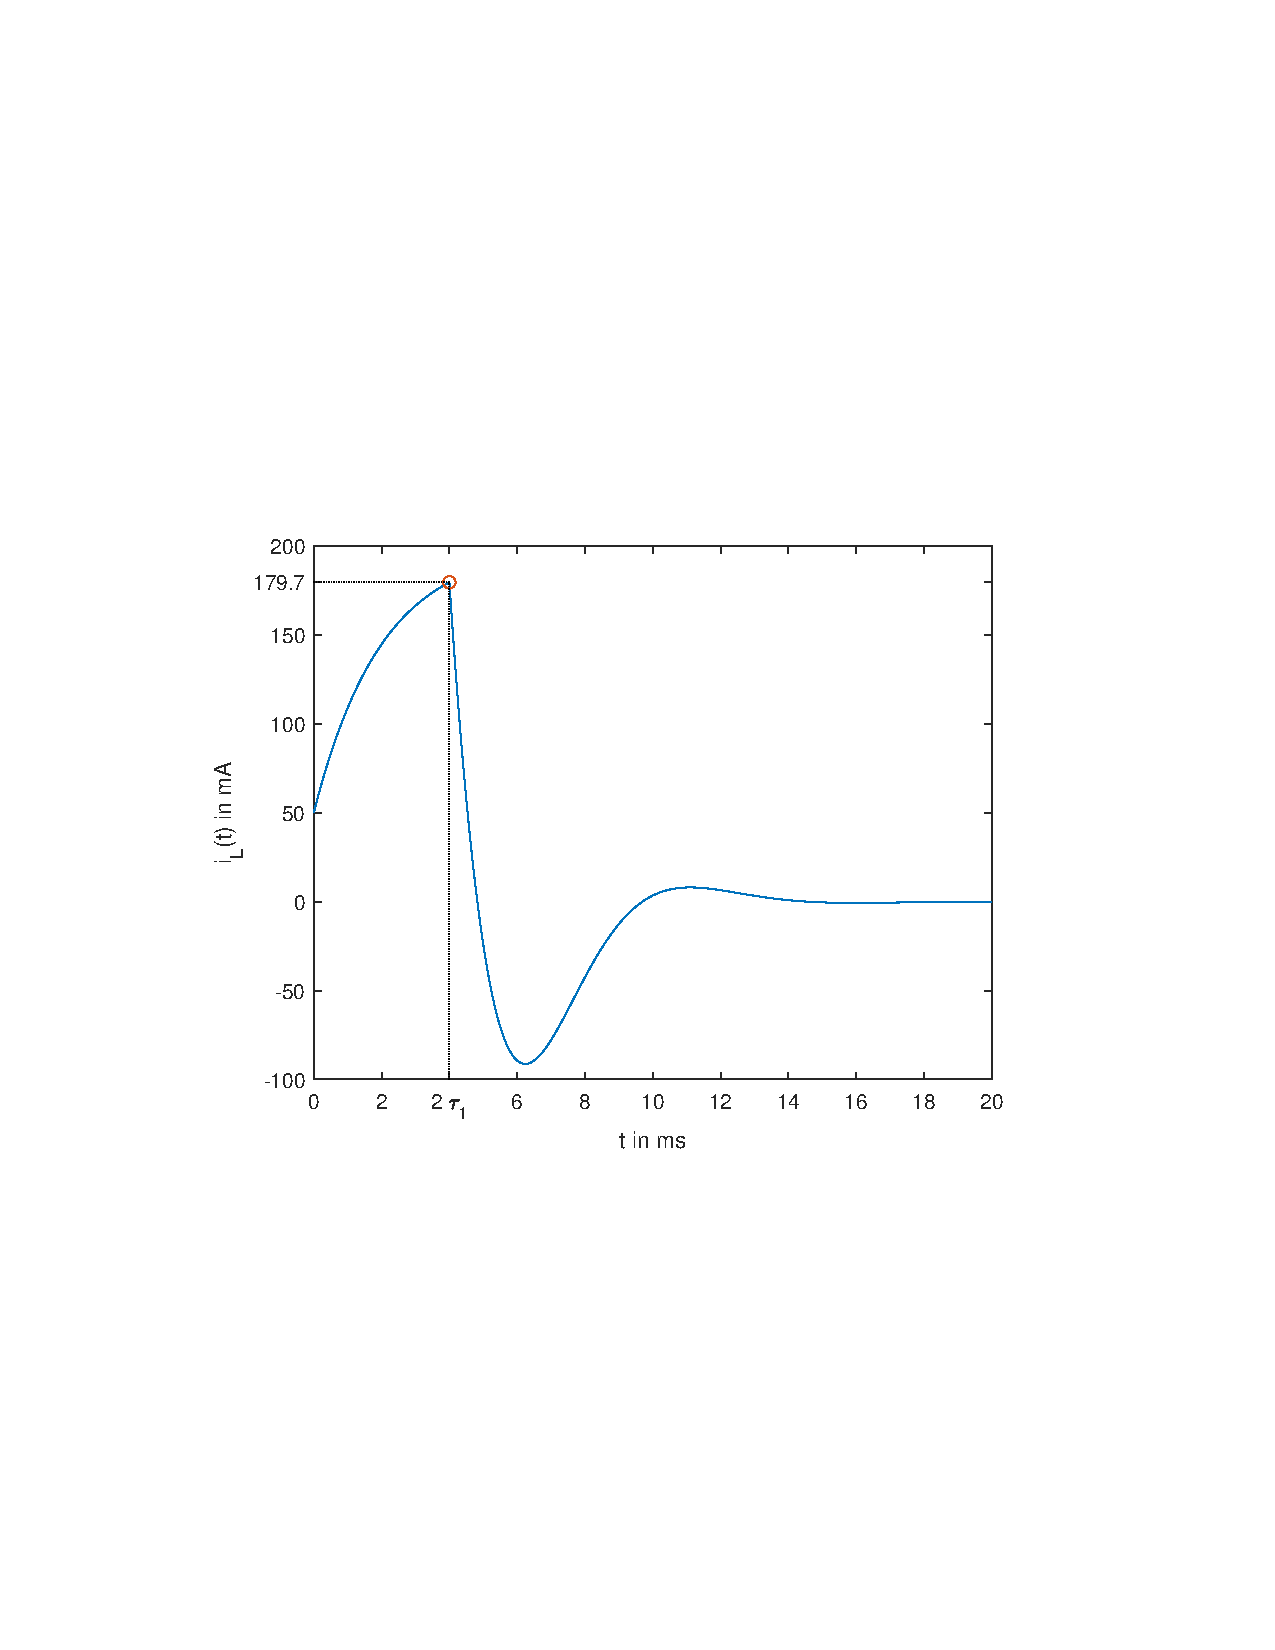
\includegraphics[width=0.70\linewidth]{./Assets/ML_Strom_Plot.pdf}
  \captionof{figure}{Matlab-Plot des Stroms $i_L(t)$}
  \label{fig:ML_Strom_Plot}
\end{center}

\begin{center}

  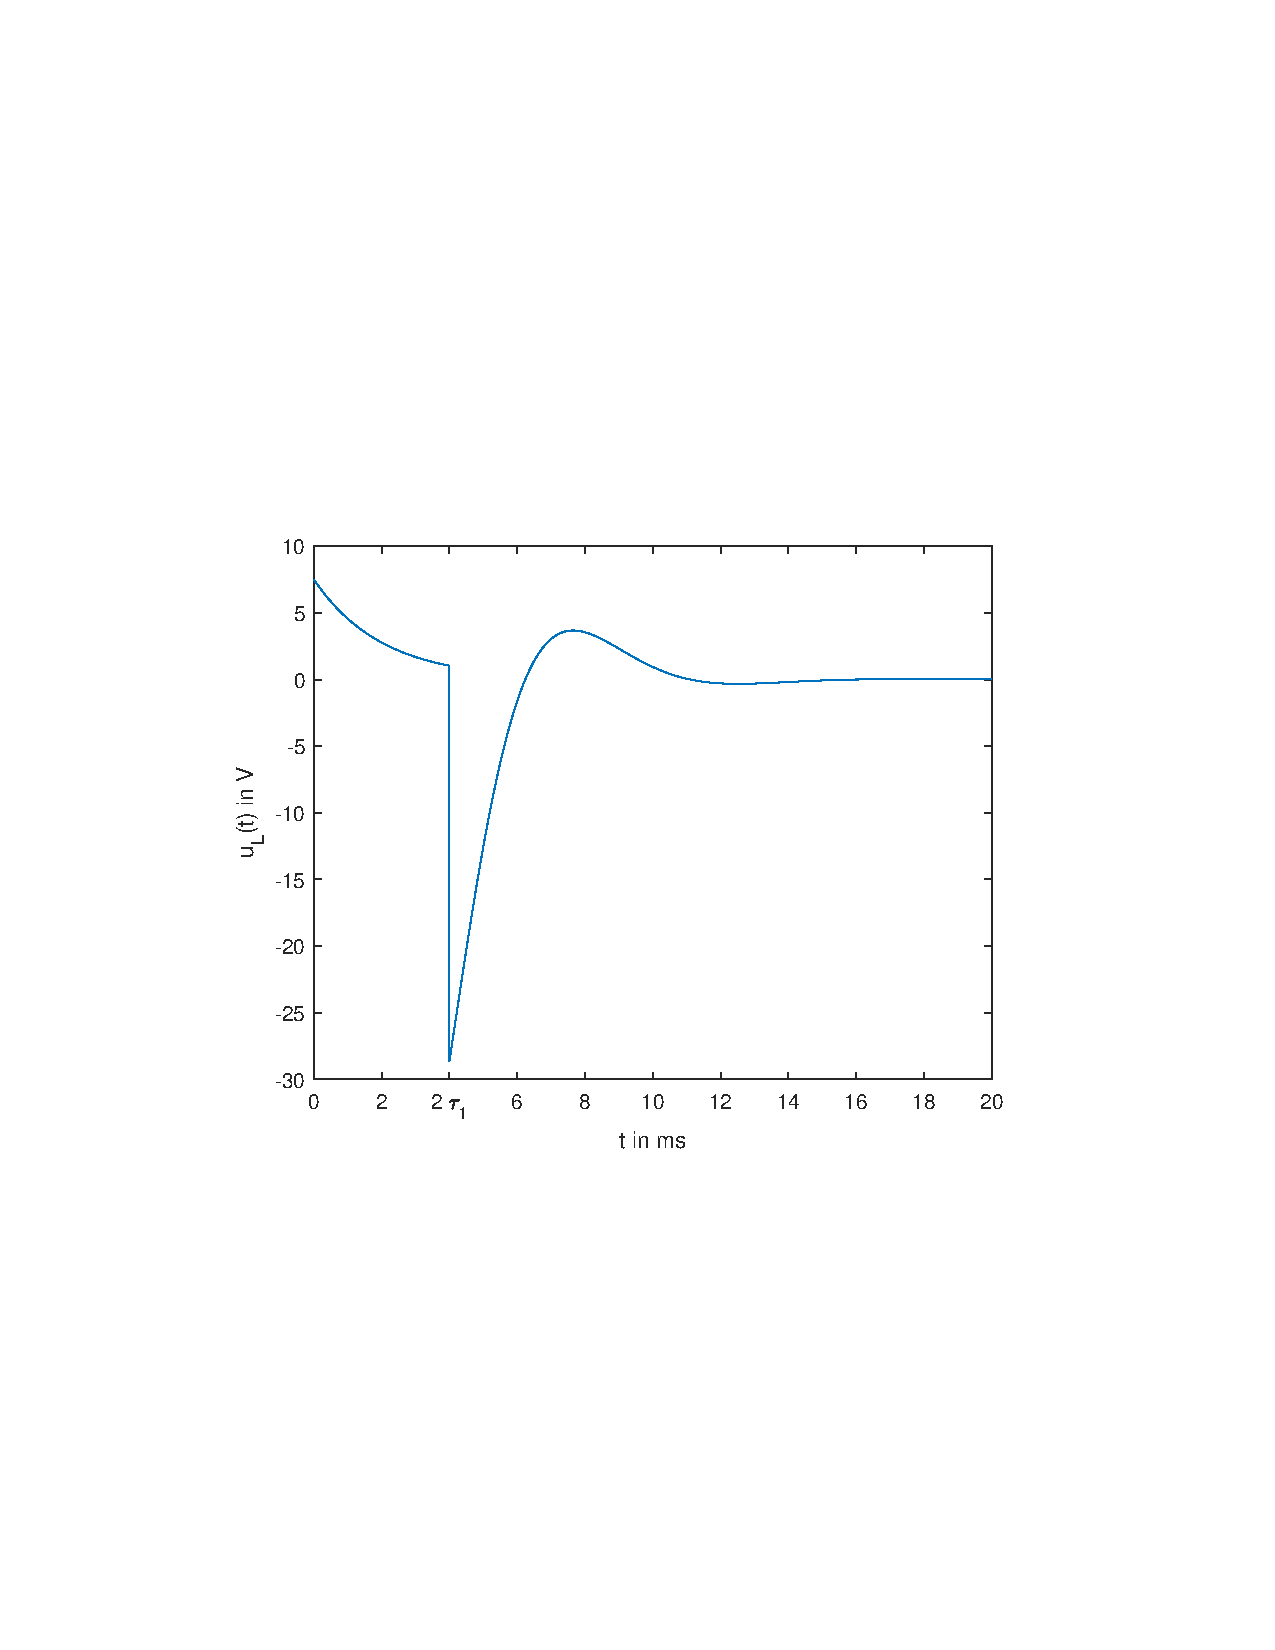
\includegraphics[width=0.70\linewidth]{./Assets/ML_Spannung_Plot.pdf}
  \captionof{figure}{Matlab-Plot der Spannung $u_L(t)$}
  \label{fig:ML_Spannung_Plot}
\end{center}

\subsection{PSpice-Plot $i_L(t)$ und $u_L(t)$} %David

% \begin{center}

  \hspace{-2cm}
  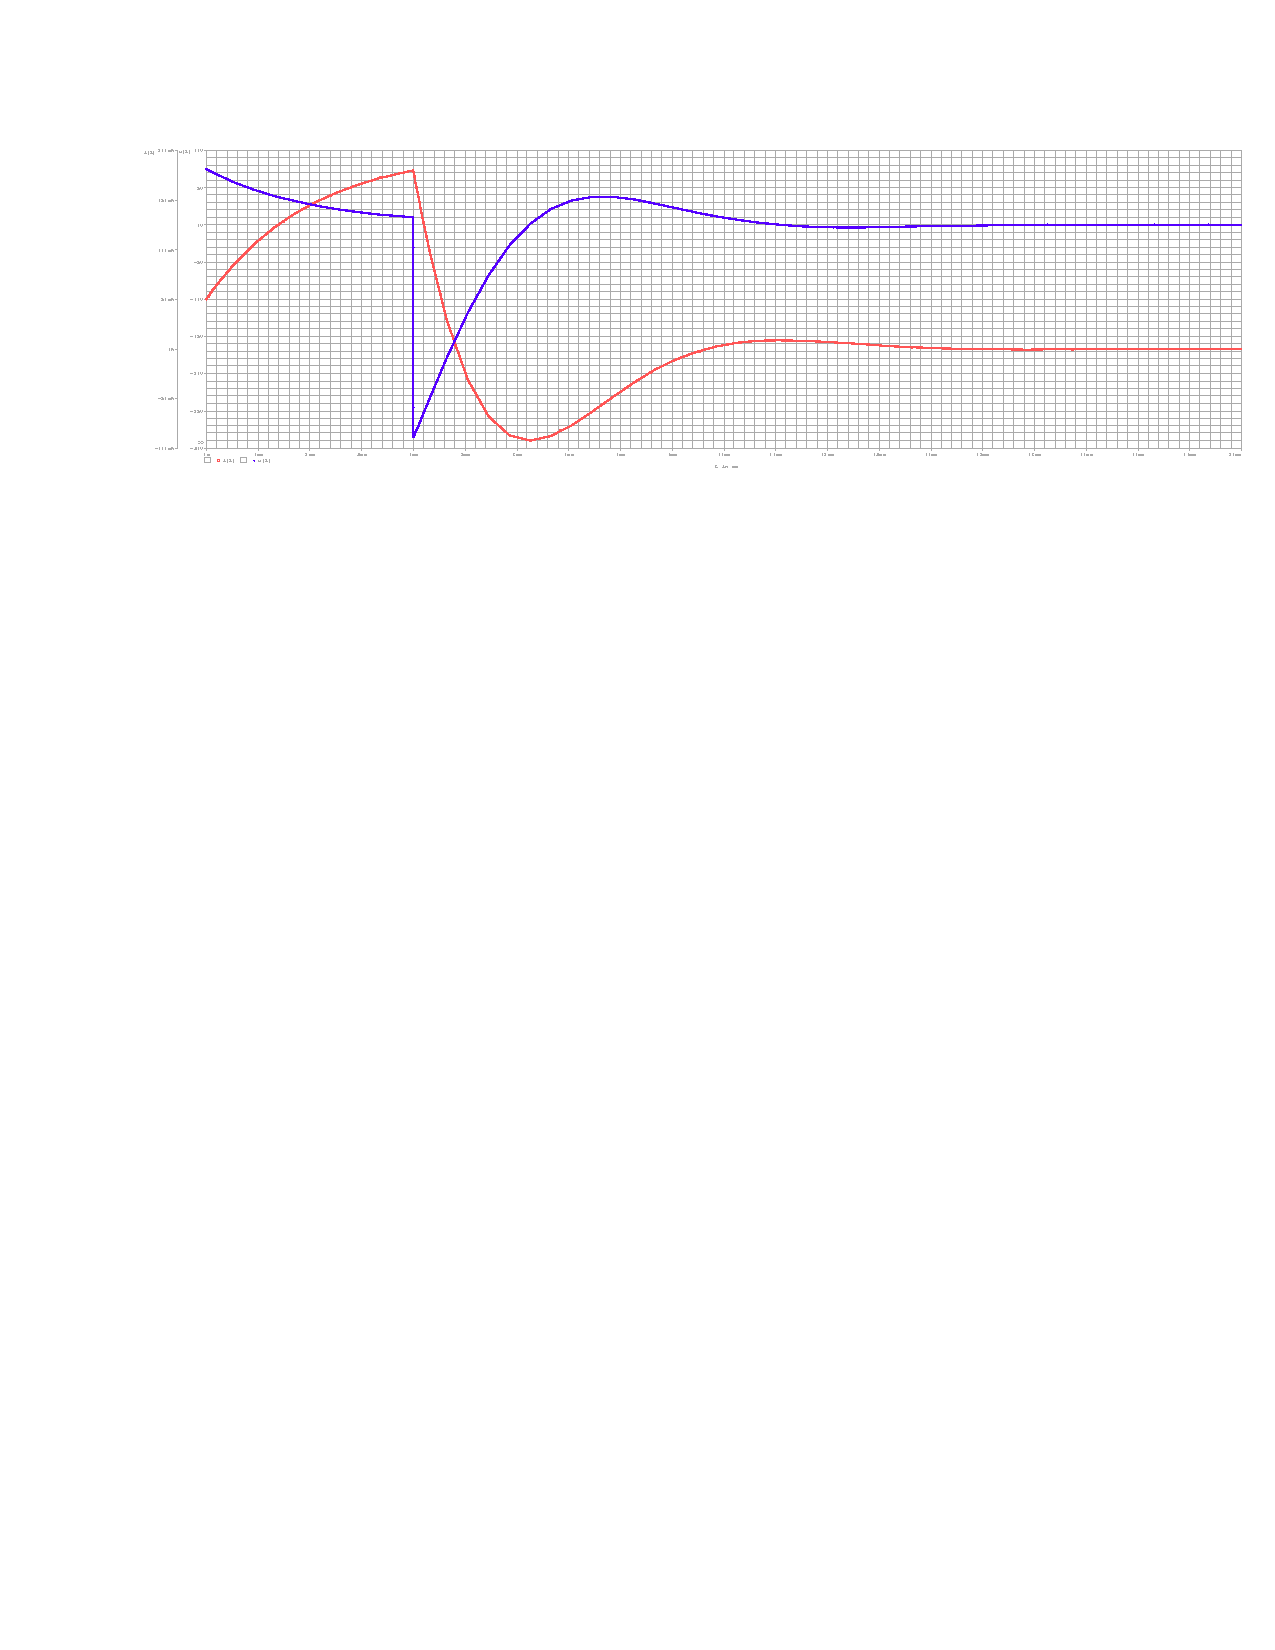
\includegraphics[width=1.25\linewidth]{./Assets/PS_doppel_plot.pdf}
  \captionof{figure}{PSpice-Plot von $i_{L}(t)$ und $u_{L}(t)$}
  \label{fig:ML_Strom_Plot}
% \end{center}
-

\end{document}
